\documentclass[13pt]{article}
\usepackage[utf8]{vietnam}
\usepackage[paperheight=29.7cm,paperwidth=21cm,right=2cm,left=3.5cm,top=3.5cm,bottom=3cm]{geometry}
\usepackage[table,xcdraw]{xcolor}
\usepackage{changepage}
\usepackage{indentfirst} % Thư viện thụt đầu dòng
\usepackage{graphicx}
\usepackage{subfig}
\usepackage{natbib}
\usepackage{color}
\usepackage{titlesec} 
\usepackage{amsmath}
\usepackage{amsfonts}
\usepackage{amssymb}
\usepackage{multirow}
\usepackage{indentfirst}
\usepackage{array}
\usepackage{indentfirst} % Thư viện thụt đầu dòng
\usepackage{graphicx}
\usepackage{booktabs}
\usepackage{placeins}
\usepackage{cite}
\usepackage{natbib}
\usepackage{enumitem}
\usepackage{hyperref}
\usepackage{color}
\usepackage{titlesec}
\counterwithin{table}{section}
\usepackage{lipsum}





\usepackage{titlesec} 
\usepackage{fancyhdr} 
\usepackage{lipsum} 
\usepackage[utf8]{vietnam}
\usepackage{placeins}


%\titlespacing*{\subsection}{0pt}{6pt}{0pt} % Heading 2
\titleformat*{\subsection}{\fontsize{16pt}{0pt}\selectfont \bfseries}
\titleformat*{\subsubsection}{\fontsize{14pt}{0pt}\selectfont \bfseries}
\renewcommand{\baselinestretch}{1.4} % Giãn dòng 1.5
\setlength{\parskip}{0.3pt} % Spacing after
\setlength{\parindent}{0.5cm} % Set khoảng cách thụt đầu dòng mỗi đoạn
\title{empty}
%\author{Trần Thị Anh Thư}
\renewcommand\thesection{\arabic{section}}




\begin{document}


%trang bia chinh
\pagenumbering{gobble}
	\fontsize{14pt}{20pt}\selectfont
	\begin{center}
		TÔNG LIÊN ĐOÀN LAO ĐỘNG VIỆT NAM\\\textbf{TRƯỜNG ĐẠI HỌC TÔN ĐỨC THẮNG}
        \\{KHOA CÔNG NGHỆ THÔNG TIN}\\

	\end{center}
	%\maketitle
	\vspace{1cm}
	\begin{figure}[h]
		\centering
		\includegraphics[width=0.3\linewidth]{image/Logo.png}
	\end{figure}
	\vspace{-1cm}
	\vspace{1cm}

\fontsize{14pt}{20pt}\selectfont
	\begin{center}
		\textbf{TRẦN THỊ ANH THƯ - 52100489 } 
        \\	
	\end{center}
    \vspace{1cm}

    
	\fontsize{24pt}{20pt}\selectfont
	\begin{center}
		\textbf{CẤU HÌNH SƠ ĐỒ MẠNG}
	\end{center}
	\vspace{1cm}
	\fontsize{22pt}{20pt}\selectfont
	\begin{center}
		\textbf{\textbf{BÁO CÁO CUỐI KỲ }\\\textbf{ MẠNG MÁY TÍNH NÂNG CAO }}	
	\end{center}
    \vspace{2cm}
	\fontsize{16pt}{20pt}\selectfont
	
	\vspace{4cm}
	\fontsize{14pt}{20pt}\selectfont
	\begin{center}
		\textbf{HỒ CHÍ MINH – 2025}
	\end{center}













\newpage
	\pagenumbering{gobble}
	\fontsize{14pt}{20pt}\selectfont
	\begin{center}
		TÔNG LIÊN ĐOÀN LAO ĐỘNG VIỆT NAM\\\textbf{TRƯỜNG ĐẠI HỌC TÔN ĐỨC THẮNG}
        \\{KHOA CÔNG NGHỆ THÔNG TIN}\\
	\end{center}
	%\maketitle
	\vspace{1cm}
	\begin{figure}[h]
		\centering
		\includegraphics[width=0.3\linewidth]{image/Logo.png}
	\end{figure}
	\vspace{-1cm}
	\vspace{1cm}

    \fontsize{14pt}{20pt}\selectfont
	\begin{center}
		\textbf{TRẦN THỊ ANH THƯ - 52100489 } 
        \\	
	\end{center}
    \vspace{1cm}
    
	\fontsize{24pt}{20pt}\selectfont
	\begin{center}
		\textbf{CẤU HÌNH SƠ ĐỒ MẠNG}
	\end{center}
	\vspace{1cm}
	\fontsize{22pt}{20pt}\selectfont
	\begin{center}
		\textbf{\textbf{BÁO CÁO CUỐI KỲ }\\\textbf{ MẠNG MÁY TÍNH NÂNG CAO  }}	
	\end{center}
    \vspace{2cm}
	\fontsize{16pt}{20pt}\selectfont
	\begin{center}
		\textbf{\textbf{\textit{Người hướng dẫn:\\ }\textbf{Giảng viên Ths. Lê Viết Thanh } 
        }\\}	
	\end{center}
	\vspace{3cm}
	\fontsize{14pt}{20pt}\selectfont
	\begin{center}
		\textbf{HỒ CHÍ MINH – 2025}
	\end{center}


%LỜI CẢM ƠN
\section*{\centering LỜI CẢM ƠN}
    \addcontentsline{toc}{section}{\numberline{} LỜI CẢM ƠN}
Em xin chân thành gửi lời cảm ơn đến thầy Lê Viết Thanh đã giúp đỡ, hướng dẫn em trong quá trình học tập và tìm hiểu về bộ môn “Mạng máy tính nâng cao”. Nhờ như vậy, em có thể thực hiện bài báo cáo này một cách tốt nhất và có thể đạt được một kết quả trọn vẹn. Một lần nữa, em xin bày tỏ lòng biết ơn của mình đến với thầy và chúc thầy sẽ luôn thành công trên con đường dạy học và nghiên cứu của mình.

Bài làm của em là sản phẩm của những sinh viên ít kinh nghiệm nên chắc hẳn còn nhiều thiếu sót. Em rất chân thành đón nhận tất cả các ý kiến đóng góp của thầy. Nhờ những ý kiến đóng góp của thầy mà các bài làm sau của em sẽ đạt được sự hoàn thiện cao hơn.
Em xin chân thành cảm ơn!



\newpage
%LỜI CAM KẾT
\section*{\centering CÔNG TRÌNH ĐƯỢC HOÀN THÀNH\\TẠI TRƯỜNG ĐẠI HỌC TÔN ĐỨC THẮNG}

Tôi xin cam đoan đây là công trình nghiên cứu của riêng tôi và được sự hướng dẫn khoa học của ThS. Lê Viết Thanh. Các nội dung nghiên cứu, kết quả trong đề tài này là trung thực và chưa công bố dưới bất kỳ hình thức nào trước đây. Những số liệu trong các bảng biểu phục vụ cho việc phân tích, nhận xét, đánh giá được chính tác giả thu thập từ các nguồn khác nhau có ghi rõ trong phần tài liệu tham khảo.
 
\textbf{Nếu phát hiện có bất kỳ sự gian lận nào tôi xin hoàn toàn chịu trách nhiệm về nội dung Báo cáo Dự án Công nghệ thông tin của mình}. Trường Đại học Tôn Đức Thắng không liên quan đến những vi phạm tác quyền, bản quyền do tôi gây ra trong quá trình thực hiện (nếu có).
\begin{center}
    \textit{
        \hspace*{7cm}Hồ Chí Minh, ngày 7 tháng 5 năm 2025 \\
        \hspace*{7cm}Tác giả\\
        \hspace*{7cm}(Ký và ghi rõ họ tên)\\
        \vspace*{0.2cm}
        \vspace*{1cm}
        \hspace*{7cm}Trần Thị Anh Thư
        }
\end{center}



   %muc luc 
	\newpage
	\tableofcontents
	\newpage
	\pagenumbering{arabic}
	\setcounter{page}{1}


%DANH MỤC KÝ HIỆU VÀ CHỮ VIẾT TẮT
\section*{\centering DANH MỤC CÁC CHỮ VIẾT TẮT}
\phantomsection
\addcontentsline{toc}{section}{\numberline {}DANH MỤC CÁC CHỮ VIẾT TẮT}

\begin{tabbing}
\hspace{1cm} \= \hspace{4cm} \= \kill
\hspace{1cm} ACL \> \hspace{4cm} Access Control List \\
\hspace{1cm} CHAP \> \hspace{4cm} Challenge Handshake Authentication Protocol \\
\hspace{1cm} DNS \> \hspace{4cm} Domain Name System \\
\hspace{1cm}  DHCP \> \hspace{4cm} Dynamic Host Configuration Protocol  \\
\hspace{1cm} EIGRP \> \hspace{4cm} Enhanced Interior Gateway Routing Protocol \\
\hspace{1cm} FTP \> \hspace{4cm} File Transfer Protocol \\
\hspace{1cm} IP \> \hspace{4cm} Internet Protocol \\
\hspace{1cm} LAN \> \hspace{4cm} Local Area Network \\
\hspace{1cm} MAC \> \hspace{4cm} Media Access Control \\
\hspace{1cm} NAT \> \hspace{4cm} Network Address Translation \\
\hspace{1cm} OSPF \> \hspace{4cm} Open Shortest Path First \\
\hspace{1cm} PPP \> \hspace{4cm} Point-to-Point Protocol \\
\hspace{1cm} SSH \> \hspace{4cm} Secure Shell \\
\hspace{1cm} TCP \> \hspace{4cm} Transmission Control Protocol \\
\hspace{1cm} UDP \> \hspace{4cm} User Datagram Protocol \\
\hspace{1cm} VLAN \> \hspace{4cm} Virtual Local Area Network \\
\end{tabbing}

\newpage
%DANH MỤC HÌNH VÀ BẢNG BIỂU
\section*{\centering DANH MỤC HÌNH ẢNH, BẢNG BIỂU}
\phantomsection
\addcontentsline{toc}{section}{DANH MỤC HÌNH ẢNH, BẢNG BIỂU}


\newpage
\begin{center}
		\textbf{TÓM TẮT}
	\end{center}

Báo cáo này tập trung vào việc triển khai mạng theo yêu cầu, cấu hình PPP, giao thức, DHCP...

Đề tài này trình bày chi tiết về việc thiết kế, cấu hình và triển khai mạng cho trụ sở chính (HQ) và chi nhánh, bao gồm:

- Phân bổ địa chỉ IPv4 và IPv6 cho các VLAN, router và thiết bị.

- Cấu hình PPP (PAP/CHAP) giữa các router.

- Triển khai định tuyến EIGRP (HQ) và OSPF (chi nhánh) cùng với việc phân phối lại tuyến.

- Cấu hình chuyển mạch (Rapid PVST+ và EtherChannel).

- Triển khai NAT và DHCP để cung cấp kết nối Internet và địa chỉ IP động.

- Triển khai IPv6, bao gồm định tuyến EIGRPv6 và phân bổ địa chỉ.


	

\newpage
        \section{MÔ TẢ ĐỀ TÀI}
        \subsection{Giới thiệu đề tài}
        \textbf{Phần 1 - Báo cáo về sơ đồ và địa chỉ mạng:}

Trình bày sơ đồ địa chỉ mạng của khu vực trụ sở chính (HQ) và chi nhánh, sử dụng các địa chỉ mạng được phân phối cho các router và các thiết
bị kết nối. Mô tả chi tiết cách phân bổ địa chỉ IP cho các VLAN
trong khu vực trụ sở chính và chi nhánh, bao gồm các thông số như
subnet mask/prefix, các địa chỉ gateway, và các địa chỉ IP cho các
máy chủ trong VLAN. Phân tích các yêu cầu về số lượng máy chủ
cho từng VLAN tại trụ sở chính và chi nhánh, và cách bạn sẽ phân
bổ IP để đáp ứng các yêu cầu này.

Báo cáo về Cấu hình PPP Mô tả chi tiết cách cấu hình kết nối PPP
giữa các router (R7 <-> R6 và R7 <-> R8), sử dụng các phương pháp
xác thực PAP và CHAP. Trình bày các bước cấu hình PPP và các
yêu cầu cần thiết để thiết lập các kết nối PPP thành công giữa các
router, cũng như các thông số cấu hình cần lưu ý
\\
		\textbf{Phần 2 - Báo cáo về Định tuyến và Cấu hình Giao thức, Chuyển Mạch và EtherChannel, về Cấu hình NAT và DHCP:}

Mô tả các bước cấu hình giao thức định tuyến EIGRP cho khu vực HQ và OSPF cho chi nhánh, bao gồm các bước phân phối lại các tuyến EIGRP vào miền OSPF và ngược lại.

Mô tả cách cấu hình chuyển mạch trong hệ thống, bao gồm việc
thay đổi giao thức Spanning Tree sang chế độ Rapid PVST+ và
cấu hình các root bridge cho các VLAN. Trình bày chi tiết cấu
hình EtherChannel với giao thức LACP cho tất cả các kết nối giữa
các switch.

Cấu hình NAT Overload trên router Access để cho phép các địa chỉ
IP riêng của HQ và chi nhánh có thể truy cập Internet. Trình bày
cách cấu hình DHCP server trên router R4 để phân phối địa chỉ IP
cho các VLAN, cũng như các tham số cần thiết cho các host\\
\textbf{Phần 3 - Báo cáo về Sơ đồ Địa chỉ IPv6 và Cấu hình EIGRP cho IPv6, Cấu hình Stateless DHCPv6 và Cấu hình Relay Agent}

Sơ đồ địa chỉ IPv6 cho các kết nối giữa các router, bao gồm việc phân
bổ địa chỉ từ mạng 2019:ABBA:CDDC:/48 cho năm VLAN khác
nhau.

Trình bày cách cấu hình giao thức EIGRP cho IPv6 tại site HQ và
các yêu cầu cấu hình để giao thức này hoạt động chính xác trong
môi trường IPv6. Giải thích cách cấu hình route mặc định từ R5
đến router Access và cách truyền bá nó vào quá trình EIGRP.

Mô tả cách cấu hình Stateless DHCPv6 trên router
R7 để cấp phát địa chỉ IP và các tham số khác cho các VLAN 10,
20, 30, và 40. Trình bày chi tiết cách cấu hình relay agent trên các
giao diện thích hợp để đảm bảo việc truyền tải thông tin DHCPv6
đúng cách.



\subsection{1.2 Mô tả sơ đồ mạng}
\textbf{(a) Tổng quan kiến trúc:}

Sơ đồ mạng được chia thành hai khu vực chính:

- BRANCH (Chi nhánh)
        
- HQ (Trụ sở chính)

Hai khu vực này được kết nối với nhau thông qua các router trung gian và có sử dụng kết nối VPN (GRE Tunnel) để đảm bảo tính bảo mật và ổn định của đường truyền.
            


\textbf{(b) Khu vực BRANCH:}
Gồm các router: R1, R2, R3

Kết nối với hai khu vực OSPF:

- Area 1: chứa các địa chỉ loopback Lo0, Lo1 của R1.

- Area 3: chứa các địa chỉ loopback Lo0, Lo1 của R3.

Các router R1 và R3 kết nối đến router trung tâm R5.


\textbf{(c) Router trung gian R5:}
Đóng vai trò là điểm kết nối giữa BRANCH và HQ.

Có kết nối:

- Với một router truy cập Internet (ký hiệu "Access", biểu tượng cloud).

- Với các router R1 và R3 ở phía BRANCH.

- Với router R4 ở phía HQ.

Có thể là điểm định tuyến trung tâm hoặc thực hiện NAT, bảo mật hoặc quản lý lưu lượng truy cập Internet.



\textbf{Khu vực HQ}
Bao gồm các router: R4, R6, R7, R8 và hệ thống switch S1 đến S4 tạo thành một mạng chuyển mạch nội bộ (LAN switching).

Các kết nối nổi bật:

- R4 kết nối với R5 (từ BRANCH).

- R4 kết nối với switch S1.

- S1, S2, S3, S4 tạo thành một mô hình vuông, đại diện cho một kiến trúc Layer 2 Switched Network, có thể dùng cho mạng nội bộ doanh nghiệp hoặc hệ thống datacenter.

- S4 kết nối với R7.

- R7 có hai nhánh kết nối đến:

- R6: đại diện cho một LAN (LAN R6).

- R8: đại diện cho một LAN khác (LAN R8), thông qua một GRE Tunnel.

- GRE Tunnel biểu thị một kết nối VPN được mã hóa qua Internet, đảm bảo dữ liệu được truyền an toàn giữa hai điểm.


\textbf{Các thiết bị đặc biệt}

- GRE Tunnel (Generic Routing Encapsulation): Nằm giữa R7 và R8. Cho phép truyền dữ liệu giữa HQ và các nhánh từ xa qua Internet bằng cách "đóng gói" các gói dữ liệu.

- LAN R6 và LAN R8: Đại diện cho hai mạng nội bộ kết nối với hai router R6 và R8. Có thể là mạng máy trạm, máy chủ hoặc thiết bị đầu cuối người dùng.



        \section{CƠ SỞ LÝ THUYẾT}
\subsection{Mạng cục bộ LAN - Local Area Network}

Mạng cục bộ được thiết kế để kết nối các máy tính thành một hệ thống mạng nội bộ, giúp việc trao đổi thông tin và chia sẻ tài nguyên trong các cơ quan hoặc doanh nghiệp trở nên dễ dàng hơn. Có hai loại mạng
LAN chính: LAN có dây và LAN không dây. Một số đặc điểm cơ bản của mạng cục bộ bao gồm:
- Quy mô mạng nhỏ: Phạm vi hoạt động của mạng LAN thường giới hạn trong vài km, kết nối các máy
tính trong cùng một tòa nhà hoặc doanh nghiệp. Quá trình quản lý và bảo trì mạng cũng đơn giản hơn so
với các loại mạng khác.
- Công nghệ truyền dẫn: Mạng LAN thường sử dụng công nghệ quảng bá, với một cáp đơn kết nối tất cả
các máy tính. Tốc độ truyền dữ liệu rất cao, từ 10 đến 100 Mbps, thậm chí có thể đạt tới hàng trăm Gbps,
với thời gian trễ rất thấp (khoảng 10 miro giây) và độ tin cậy cao, tỷ lệ lỗi bit dao động từ 10−8 đến 10−11.
- Cấu trúc topo mạng: Mạng LAN có thể được cấu trúc theo nhiều hình thức khác nhau, như hình BUS,
vòng (Ring), hình sao (Star), hoặc các cấu trúc kết hợp, lai ghép...
          

        \subsection{Khái niệm các loại giao thức thực hiện trong bài:}

\textbf{PPP và CHAP:}

PPP là viết tắt của Point-to-Point Protocol, một giao thức Layer 2 (Data Link Layer) được sử dụng để thiết lập một kết nối trực tiếp giữa hai nút mạng (thường là qua đường dây serial hoặc dial-up).

Tính năng chính của PPP:

- Hỗ trợ xác thực (Authentication).

- Đóng gói nhiều loại giao thức Layer 3 (IPv4, IPv6...).

- Phát hiện lỗi (Error detection).

- Nén dữ liệu (optional).

- Đàm phán cấu hình đường truyền (qua LCP – Link Control Protocol).

CHAP là một phương thức xác thực trong PPP. Nó an toàn hơn so với PAP vì không truyền mật khẩu dưới dạng văn bản rõ ràng.

Cách CHAP hoạt động:

- Khi kết nối PPP được thiết lập, máy chủ (authenticator) gửi một thách thức (challenge) ngẫu nhiên tới máy khách.

- Máy khách phản hồi bằng cách băm mật khẩu và challenge này.

- Máy chủ so sánh với giá trị băm dự kiến. Nếu trùng khớp → xác thực thành công.

CHAP có thể gửi lại challenge bất kỳ lúc nào trong suốt phiên để xác thực liên tục.


\textbf{EIGRP và OSPF:}
EIGRP là một giao thức định tuyến hybrid (lai giữa distance-vector và link-state) được Cisco phát triển độc quyền, hoạt động chủ yếu trong hệ thống Autonomous System nội bộ.

Đặc điểm nổi bật của EIGRP:

- Giao thức lai: Kết hợp ưu điểm của cả distance-vector và link-state.

- Sử dụng DUAL algorithm (Diffusing Update Algorithm) để đảm bảo không có vòng lặp.

- Hỗ trợ tốc độ hội tụ nhanh.

- Gửi cập nhật không định kỳ (chỉ khi có thay đổi).

- Sử dụng số liệu composite metric (bao gồm bandwidth, delay, reliability, load).

- Hỗ trợ VLSM, CIDR và IPv4/IPv6.


OSPF là một giao thức định tuyến link-state tiêu chuẩn mở (open standard), được sử dụng rộng rãi trong các hệ thống mạng lớn.

Đặc điểm nổi bật của OSPF:

- Tiêu chuẩn mở – hỗ trợ nhiều nhà sản xuất thiết bị.

- Sử dụng thuật toán Dijkstra (SPF – Shortest Path First).

- Chia mạng thành Areas để dễ quản lý, trong đó Area 0 là Backbone.

- Hỗ trợ VLSM, CIDR, Load balancing, và authentication.

- Cập nhật định kỳ bằng LSA (Link-State Advertisement).

- Tốc độ hội tụ rất nhanh.


\textbf{NAT và DHCP:}

NAT là viết tắt của Network Address Translation, nghĩa là chuyển đổi địa chỉ IP giữa mạng nội bộ (private) và mạng bên ngoài (public – Internet).

Mục đích của NAT:

-Tiết kiệm địa chỉ IPv4 công cộng.

-Ẩn địa chỉ IP nội bộ, tăng tính bảo mật.

- Cho phép nhiều thiết bị nội bộ truy cập Internet qua một địa chỉ IP công cộng duy nhất.



DHCP là viết tắt của Dynamic Host Configuration Protocol, là giao thức dùng để tự động cấp phát thông tin cấu hình IP cho các thiết bị trong mạng, như:

- Địa chỉ IP

- Subnet mask

- Default gateway








\newpage
\section{MÔ HÌNH HỆ THỐNG}
\subsection{Sơ đồ luận lý}

       \begin{figure}[h!]
                \centering
                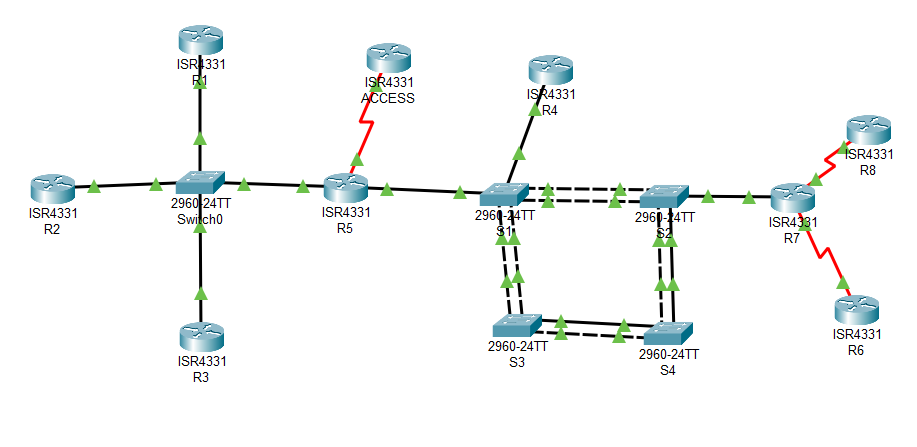
\includegraphics[width=1.0\linewidth]{sodo1.png}
                \caption{So do luan ly}
            \end{figure}
            

    \subsection{Sơ đồ vật lý}

  \begin{figure}[h!]
                \centering
                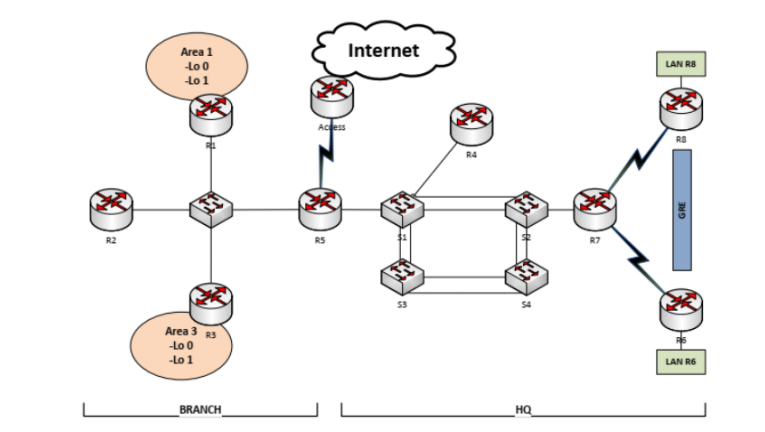
\includegraphics[width=1.0\linewidth]{sodo2.png}
                \caption{EVE}
            \end{figure}
    
\newpage
    \section{THÔNG TIN CÀI ĐẶT HỆ THỐNG}
    \subsection{Thông tin vlan, interface vlan trong hệ thống}
\textbf{Chia IPv4 cho các subnet hệ thống mạng}

Dùng dải địa chỉ IPv4 : 7.0.0.0/8

\linewidth

		\begin{table}[]
		  \centering
		  \begin{tabular}{|>{\raggedright\arraybackslash}m{4.0cm}|>{\raggedright\arraybackslash}m{2.0cm}|>
          {\raggedright\arraybackslash}m{3.0cm}|>
          {\raggedright\arraybackslash}m{2.5cm}|}
            \hline
            
	       \textbf{Subnet} & \textbf{VLAN} & \textbf{Address } & \textbf{Subnet Mask} \\
            \hline
		      \textbf{UNIT1} & 10 & 7.0.2.0 & /24\\
            \hline
                \textbf{UNIT2} & 20 & 7.0.0.0 & /23 \\
            \hline
                \textbf{UNIT3} & 30 & 7.0.3.0 &/25 \\
                
            \hline
                \textbf{GUEST} & 40 & 7.0.3.128 & /26\\
            \hline
                \textbf{SERVERS} & 50 & 7.0.3.192 & /28\\
            \hline
                \textbf{Management(Native)} & 60  & 7.0.3.192 & /27\\
            \hline


		  \end{tabular}

\caption{Bảng thông tin chia không gian địa chỉ IPv4 cho các subnet.}
            \label{tab:my_label}
		\end{table}


		\begin{table}[]
		  \centering
		  \begin{tabular}{|>{\raggedright\arraybackslash}m{2.5cm}|>{\raggedright\arraybackslash}m{3.5cm}|>
          {\raggedright\arraybackslash}m{3.5cm}|>
          {\raggedright\arraybackslash}m{3cm}|}
            \hline
            
	       \textbf{VLAN} & \textbf{IP range} & \textbf{Broadcast } & \textbf{IP usable } \\
            \hline
		      \textbf{10} & 7.0.2.1 - 7.0.2.254 & 7.0.2.255 & /252\\
            \hline
                \textbf{20} & 7.0.0.1 - 7.0.1.254 & 7.0.1.255 & /252 \\
            \hline
                \textbf{30} & 7.0.3.1 - 7.0.3.126 & 7.0.3.127 &/252 \\
                
            \hline
                \textbf{40} & 7.0.3.129 - 7.0.3.190& 7.0.3.191 & /252\\
            \hline
                \textbf{50} & 7.0.3.193 - 7.0.3.222 & 7.0.3.239 & /252\\
            \hline
                \textbf{60} & 7.0.3.225 - 7.0.3.238  & 7.0.3.223 & /252\\
            \hline


		  \end{tabular}
\caption{Yêu cầu về số lượng máy chủ cho chi nhánh}
            \label{tab:my_label}
		\end{table}


\begin{table}[]
		  \begin{tabular}{|>{\raggedright\arraybackslash}m{2.5cm}|>{\raggedright\arraybackslash}m{2cm}|>
          {\raggedright\arraybackslash}m{3cm}|>
          {\raggedright\arraybackslash}m{3cm}|>{\raggedright\arraybackslash}m{3cm}|}
            \hline
            
	       \textbf{Thiết bị} & \textbf{Interface} & \textbf{Dải địa chỉ } & \textbf{ Host available} & \textbf{Host} \\
            
            \hline
 \textbf{R1} & \textbf{lo0} & \textbf{107.104.0.0 } & \textbf{510 } & \textbf{500} \\
            
            \hline
 \textbf{R1} & \textbf{lo1} & \textbf{107.104.2.0 } & \textbf{510 } & \textbf{300} \\
            
            \hline
 \textbf{R3} & \textbf{lo0} & \textbf{107.104.4.0 } & \textbf{254 } & \textbf{200} \\
            
            \hline
 \textbf{R2} & \textbf{lo0} & \textbf{107.104.5.0} & \textbf{126 } & \textbf{100} \\
            
            \hline
 \textbf{R3} & \textbf{lo1} & \textbf{107.104.5.128 } & \textbf{126 } & \textbf{100} \\
            
            \hline

		  \end{tabular}
\caption{Yêu cầu về số lượng máy chủ cho chi nhánh}
            \label{tab:my_label}
		\end{table}

   \section{CẤU HÌNH HẠ TẦNG}
  \subsection{Cấu hình Kết nối PPP, Tunneling GRE }

\begin{figure}[h!]
                \centering
                \includegraphics[width=0.5\linewidth]{image/ppp.png}
                \caption{Cấu hình PPP}
                \label{fig:label1}
            \end{figure}

\begin{figure}[h!]
                \centering
                \includegraphics[width=0.5\linewidth]{image/chap.png}
                \caption{Cấu hình CHAP}
                \label{fig:label1}
            \end{figure}

\begin{figure}[h!]
                \centering
                \includegraphics[width=0.5\linewidth]{image/gre.png}
                \caption{Cấu hình Gre}
                \label{fig:label1}
            \end{figure}

   \subsection{Định tuyến, Chuyển mạch: }
\begin{figure}[h!]
                \centering
                \includegraphics[width=0.5\linewidth]{image/r5ospf.png}
                \caption{OSPF của R5}
                \label{fig:label1}
            \end{figure}

\begin{figure}[h!]
                \centering
                \includegraphics[width=0.5\linewidth]{image/access.png}
                \caption{Cấu hình access}
                \label{fig:label1}
            \end{figure}

\begin{figure}[h!]
                \centering
                \includegraphics[width=0.5\linewidth]{image/s1.png}
                \caption{cấu hình switch chính}
                \label{fig:label1}
            \end{figure}

  \subsection{NAT và DHCP:}


\begin{figure}[h!]
                \centering
                \includegraphics[width=0.5\linewidth]{image/r41.png}
                \caption{Cấu hình router R4}
                \label{fig:label1}
            \end{figure}

\begin{figure}[h!]
                \centering
                \includegraphics[width=0.5\linewidth]{image/R42.png}
                \caption{Router r4}
                \label{fig:label1}
            \end{figure}

 \subsection{IPv6:}

\begin{figure}[h!]
                \centering
                \includegraphics[width=0.5\linewidth]{image/ipv6r5.png}
                \caption{Router R5 ipv6}
                \label{fig:label1}
            \end{figure}

\begin{figure}[h!]
                \centering
                \includegraphics[width=0.5\linewidth]{image/ipv6r7.png}
                \caption{Router r7 ipv6}
                \label{fig:label1}
            \end{figure}



\newpage
\newpage
\section{CẤU HÌNH HẠ TẦNG}
\subsection{Cấu hình cơ bản cho router, switch:} 
Trên tất cả thiết bị router, switch cấu hình:

    POPNT TO POINT
R7
en
conf t
hostname R7
int s0/1/0
ip add 200.0.100.2 255.255.255.252
no shut
clock rate 128000
end


R8
en
conf t
hostname R8
int s0/1/0
ip add 200.0.100.1 255.255.255.252
no shut

R7
en
conf t
hostname R7
int s0/1/1
ip add 200.0.100.5 255.255.255.252
no shut
clock rate 128000
end



R6
en
conf t
hostname R6
int s0/1/0
ip add 200.0.100.6 255.255.255.252
no shut

ping 200.0.100.5 lai ktra


R5

en
conf t
hostname R5
int s0/1/0
ip add 200.0.100.9 255.255.255.252
no shut

ACCESS
en
conf t
hostname ACCESS
int s0/1/0
ip add 200.0.100.10 255.255.255.252
no shut

clock rate 128000
end



DAT IP
R4

interface GigabitEthernet0/0/0
no shut 
exit

 interface GigabitEthernet0/0/0.10
 encapsulation dot1Q 10
 ip address 7.0.0.2 255.255.254.0

interface GigabitEthernet0/0/0.20
 encapsulation dot1Q 20
 ip address 7.0.2.2 255.255.255.0

interface GigabitEthernet0/0/0.30
 encapsulation dot1Q 30
 ip address 7.0.3.3 255.255.255.128

interface GigabitEthernet0/0/0.40
 encapsulation dot1Q 40
 ip address 7.0.3.130 255.255.255.192

interface GigabitEthernet0/0/0.50
 encapsulation dot1Q 50
 ip address 7.0.3.226 255.255.255.240

interface GigabitEthernet0/0/0.60
 encapsulation dot1Q 60 native
 ip address 7.0.3.194 255.255.255.224



R1 Lo0, lo1
R1(config-if)#ip add 107.104.0.0 255.255.254.0
Bad mask /23 for address 107.104.0.0
R1(config-if)#ip add 107.104.0.1 255.255.254.0
R1(config-if)#no shut
R1(config-if)#exit
R1(config)#int lo1

R1(config-if)#

R1(config-if)#ip add 107.104.2.1 255.255.254.0
R1(config-if)#exit
R1(config)#int gi0/0/0
R1(config-if)#ip add 107.104.5.129 255.255.255.128
R1(config-if)#no shut


R2 Lo0
Router#conf t
Enter configuration commands, one per line.  End with CNTL/Z.
Router(config)#int lo0

Router(config-if)#, changed state to up

Router(config-if)#ip add 107.104.5.0 255.255.255.128
Bad mask /25 for address 107.104.5.0
Router(config-if)#ip add 107.104.5.1 255.255.255.128
Router(config-if)#exit
Router(config)#
Router(config)#
Router(config)#hostname R2
R2(config)#

R3(config-if)#
R3(config-if)#end
R3#copy running-config startup-config
Destination filename [startup-config]? 
Building configuration...


R3#
OSPF
R2#router ospf 1

R2#conf t
Enter configuration commands, one per line.  End with CNTL/Z.
R2(config)#router ospf 1
R2(config-router)#network 7.0.0.0 0.255.255.255 area 0
R2(config-router)#net 200.0.100.0 0.0.0.255 area 0
R2(config-router)#end
R2#

R2# vaf R1, R3 luon
router ospf 1
 log-adjacency-changes
 network 7.0.0.0 0.255.255.255 area 0
 network 200.0.100.0 0.0.0.255 area 0

router eigrp 100
 passive-interface GigabitEthernet0/0/0
 passive-interface GigabitEthernet0/0/0.10
 passive-interface GigabitEthernet0/0/0.20
 passive-interface GigabitEthernet0/0/0.30
 passive-interface GigabitEthernet0/0/0.40
 passive-interface GigabitEthernet0/0/0.50
 network 7.0.0.0 0.255.255.255 area 0
 network 200.0.100.0 0.0.0.255 area 0

interface GigabitEthernet0/1/0
 ip address 200.0.100.10 255.255.255.255
 ip nat inside
clock rate 128000

- SWTCH

S1(config)#vtp domain anhthu
Changing VTP domain name from NULL to anhthu
S1(config)#vtp mode server

Switch(config)#vtp domain anhthu
Changing VTP domain name from NULL to anhthu
Switch(config)#vtp mode client
Setting device to VTP CLIENT mode.

S1(config-vlan)#name UNIT2
S1(config-vlan)#vlan 30
S1(config-vlan)#name UNIT3
S1(config-vlan)#vlan 40
S1(config-vlan)#name GUEST
S1(config-vlan)#vlan 50
S1(config-vlan)#name SERVERS
S1(config-vlan)#vlan 60 
S1(config-vlan)#name Managerment(Native)
S1(config-vlan)#end

int range F0/1-4
switchport mode trunk


##Native vlan
int range F0/1-4
sw trunk native vlan 60


##soanninf tree
spanning-tree mode rapid-pvst

##S1 root vlan 10 20 30
spanning-tree mode ra
spanning-tree vlan 10 root primary
spanning-tree vlan 20 root primary
spanning-tree vlan 30 root primary


Sw2
spanning-tree mode ra
spanning-tree vlan 1 root primary
spanning-tree vlan 50 root primary
spanning-tree vlan 60 root primary


SW1
int vlan 60
ip add 7.0.3.194 255.255.255.224


sw2
int vlan 60
ip add 7.0.3.195 255.255.255.224

int vlan 60
ip add 7.0.3.196 255.255.255.224

int vlan 60
ip add 7.0.3.197 255.255.255.224


##SSH
ip domain-name anhthu.tdtu.vn
crypto key generate rsa 
module 1024
username admin pass tdtu
line vty 0 4
login local
transport input ssh



Router on a stick
ip default-gateway 7.0.3.225
S1(config)#



LInk all
4Sw
int range F0/1-2
channel-group 1 mode active
exit
int range F0/3-4
channel-group 2 mode active


NATT
ACCESS#conf t
ACCESS(config)#access-list 1 permit any
ACCESS(config)#no interface loopback 0
ACCESS(config)#
ip nat inside source list 1 int gi0/0/0 overload
ACCESS(config)#int gi0/0/0

ACCESS(config-if)#ip nat outside
ACCESS(config-if)#exit
ACCESS(config)#int s0/1/0
ACCESS(config-if)#ip nat inside


ip dhcp pool VLAN10
net 7.0.0.0 255.255.254.0
default-router 7.0.2.1
dns 8.8.8.8
exit

ip dhcp pool VLAN20
net 7.0.0.0 255.255.254.0
default-router 7.0.0.1
dns 8.8.8.8
exit

ip dhcp pool VLAN30
net 7.0.0.0 255.255.254.0
default-router 7.0.3.1
dns 8.8.8.8
exit

ip dhcp pool VLAN30
net 7.0.0.0 255.255.254.0
default-router 7.0.3.129
dns 8.8.8.8
exit



interface FastEthernet0/5
 switchport access vlan 50

interface FastEthernet0/6
 switchport access vlan 10

interface FastEthernet0/7
 switchport access vlan 20

interface FastEthernet0/8
 switchport access vlan 30

interface FastEthernet0/9
 switchport access vlan 40


-Trên R7-R5

ip access-list extended Block-Internal
deny ip any 7.0.0.0 0.255.255.255
deny ip any 107.104.0.0 0.7.255.255
permit ip any any
exit

int gi0/0/0.40 
ip access-group Block-Internal in



- IPv6

R5:

interface GigabitEthernet0/0

 ipv6 address FE80::R5A link-local
 
 ipv6 address 2019:ABBA:AAAA:1::1/64
 
 no shutdown

Trên R5 (HQ):

ipv6 unicast-routing

ipv6 router eigrp 100

 eigrp router-id 5.5.5.5
 
 no shutdown
 
- Trên các interface (ví dụ G0/0, G0/1, G0/2):

interface GigabitEthernet0/0

 ipv6 address 2019:ABBA:AAAA:1::1/64
 
 ipv6 address FE80::R5A link-local
 
 ipv6 eigrp 100
 
 no shutdown

Trên các interface (ví dụ G0/0, G0/1, G0/2):

interface GigabitEthernet0/0

 ipv6 address 2019:ABBA:AAAA:1::1/64
 
 ipv6 address FE80::R5A link-local
 
 ipv6 eigrp 100
 
 no shutdown
 
Lặp lại tương tự cho các router: R4, R6, R7, R8, dùng ipv6 router eigrp 100, và gán các interface phù hợp.

- Tạo default route và redistribute vào EIGRP trên R5

ipv6 route ::/0 2019:ABBA:AAAA:1::2  ! chỉ về Access

ipv6 router eigrp 100

 redistribute static

ipv6 router eigrp 100

 eigrp router‑id 10.10.10.10
 
interface Gig0/0.10

 ipv6 eigrp 100

interface Tunnel0

 ipv6 eigrp 100

ipv6 route ::/0 FE80::ACCESS   

ipv6 add FE80::R5A link-local


int gi0/0/0
ipv6 add 2019:ABBA:AAAA:1::1/64

Inter-VLAN Routing (trên R6/R8)

Trên R6 
interface GigabitEthernet0/1.10

 encapsulation dot1Q 10
 
 ipv6 address 2019:ABBA:CDDC:0:10::1/64
 
 ipv6 address FE80::1 link-local
 
 ipv6 eigrp 100

interface GigabitEthernet0/1.20

 encapsulation dot1Q 20
 
 ipv6 address 2019:ABBA:CDDC:0:20::1/64
 
 ipv6 address FE80::1 link-local
 
 ipv6 eigrp 100
 
- Làm tương tự cho VLAN 30, 40, 50 với subnet:

2019:ABBA:CDDC:0:30::/64

2019:ABBA:CDDC:0:40::/64

2019:ABBA:CDDC:0:50::/64

- Stateless DHCPv6 trên R7

Cấu hình pool DHCPv6:

ipv6 dhcp pool VLAN10

 dns-server 2001:4860:4860::8888
 
 domain-name vlan10.local

ipv6 dhcp pool VLAN20

 dns-server 2001:4860:4860::8888
 
 domain-name vlan20.local

interface GigabitEthernet0/1.10

 encapsulation dot1Q 10
 
 ipv6 address 2019:ABBA:CDDC:0:10::1/64
 
 ipv6 address FE80::R7V10 link-local
 
 ipv6 nd other-config-flag
 
 ipv6 dhcp server VLAN10
 
 no shutdown

interface GigabitEthernet0/0/1.10

 encapsulation dot1Q 10
 
 ipv6 address 2019:ABBA:CDDC:0:10::1/64
 
 ipv6 address FE80::R7V10 link-local
 
 ipv6 nd other-config-flag
 
 ipv6 dhcp server VLAN10
 
 no shutdown


interface GigabitEthernet0/0/1.10

 encapsulation dot1Q 10
 
 ipv6 address 2019:ABBA:CDDC:0:10::1/64
 
 ipv6 address FE80::1 link-local
 
 ipv6 eigrp 100

interface GigabitEthernet0/0/1.20

 encapsulation dot1Q 20
 
 ipv6 address 2019:ABBA:CDDC:0:20::1/64
 
 ipv6 address FE80::1 link-local
 
 ipv6 eigrp 100



    
\newpage
\subsection{Kết Quả Thực Hành}
5.1. Tại HQ
VLAN 20 (IT):

Yêu cầu: 300 host → Chọn /23 (510 host) để dư 210 IP.

Lý do: Phòng trường hợp mở rộng phòng IT.

5.2. Tại Chi nhánh
R1 lo0:

Yêu cầu: 500 host → Chọn /23 (510 host) → Dư 10 IP.

Nếu cần thêm, có thể dùng /22 (1022 host).

6. Kết luận
HQ: Sử dụng VLSM để tối ưu IPv4, kết hợp IPv6 cho kết nối router.

Chi nhánh: Dùng IPv4 cho loopback và IPv6 cho LAN.

Tính dự phòng: Subnet luôn dư 10-20

Không làm được yêu cầu cuối cùng của phần Ipv6 do Cisco chưa hỗ trợ.


Hết.\centering
\end{document}
